\section{Using continously changing parameters instead of a sharply changing parameter}

\subsection{Introduction}
Instead of using an if-statement to change the value of an ODE model's parameter, some models may use a function that mimicks the changes in parameter. The idea is to use a function such as the exponential, sigmoid, inverse sigmoid, tanh and others to change the value of parameters sharply when required. In the case of the Covid-19 ODE model, an idea to model the change in the $\beta$ parameter would be to use the inverse sigmoid scaled between 0.9 and 0.005 instead of a simple if-statement. 


In this section, we discuss using such sharply changing functions for the model parameters and show how they introduce thrashing, inaccuracy issues and some efficiency issues. We tackle both modeling a time-dependent discontinuity and a state-dependent discontinuity model with these rapidly changing functions and report on ways to improve the accuracy.

\subsubsection{Functions Used to model parameters}
\paragraph{The inverse sigmoid function}
An inverse sigmoid function defined as follows:
\begin{equation}
    \beta(t) =     \frac{0.895e^{-a*(t - t_c)}}{1 + e^{-a*(t - t_c)}} + 0.005
\end{equation}
is a function that decreases from 0.9 to 0.005 at $t_c$ with a steepness of change of $a$.
This function can be used to model the if-statement when adding Covid-19 measures at time $t_c$ and the steepness of change, $a$, models how quickly the population adapts to the introduction of these measures.

By varying the value of $a$, we can change the steepness of discontinuity. Figure $\ref{fig:exp_inverse_sigmoid}$ shows how different values of $a$ smoothed the discontinuity. We can see that a smaller value of a makes the change of the parameter $beta$ from 0.9 to 0.005 slower.

\begin{figure}[H]
\centering
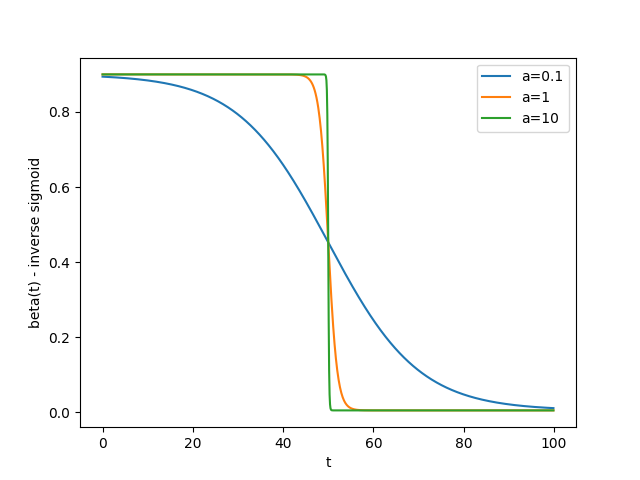
\includegraphics[width=0.7\linewidth]{./figures/exp_inverse_sigmoid}
\caption{Inverse sigmoid with discontinuity at $t_c=50$ with steepness of change, $a$, at 0.1, 1, 10.}
\label{fig:exp_inverse_sigmoid}
\end{figure}

\paragraph{The sigmoid function}
A sigmoid function defined as follows:
\begin{equation}
    \beta(t) = \frac{0.895}{(1 + e^{-a(t - t_c)}))} + 0.005
\end{equation}
is a function that increases from 0.005 to 0.9 at $t_c$ with a steepness of change of $a$.
This function can be used to model the if-statement when removing Covid-19 measures at time $t_c$ and the steepness of change, $a$, models how quickly the population adapts to removal of these measures.

By varying the value of $a$, we can change the steepness of discontinuity. Figure $\ref{fig:exp_sigmoid}$ shows how different values of $a$ smoothed the discontinuity. We can see that a smaller value of a makes the change of the parameter $beta$ from 0.005 to 0.9 slower.

\begin{figure}[H]
\centering
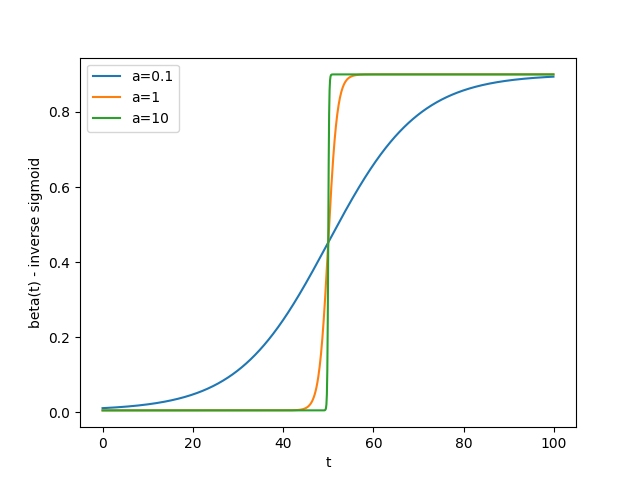
\includegraphics[width=0.7\linewidth]{./figures/exp_sigmoid}
\caption{Sigmoid with discontinuity at $t_c=50$ with steepness of change, $a$, at 0.1, 1, 10.}
\label{fig:exp_sigmoid}
\end{figure}

\subsubsection{Existence of thrashing}
In this section, we show that depending on the steepness of change, thrashing also occurs in the ODE model.

Figure $\ref{fig:exp_thrashing_lsoda}$ and $\ref{fig:exp_thrashing_dop853}$ shows the cumulative number of function evaluations at each time when solving the Covid-19 time-dependent discontinuity model using the inverse sigmoid function to model the change in the parameter $\beta$ at $t=27$ instead of using an if-statement using the `LSODA' and the `DOP853' methods of $solve\_ivp$ in Python. We can see that for small values of the steepness of change, $a$, there is no spike in the number of function evaluations at $t=27$ but as the value of $a$ is increased, a progressively sharper spike can be seen. This indicates some level of thrashing as repeated step-size reductions to cross the discontinuity was required.


\begin{figure}[H]
\centering
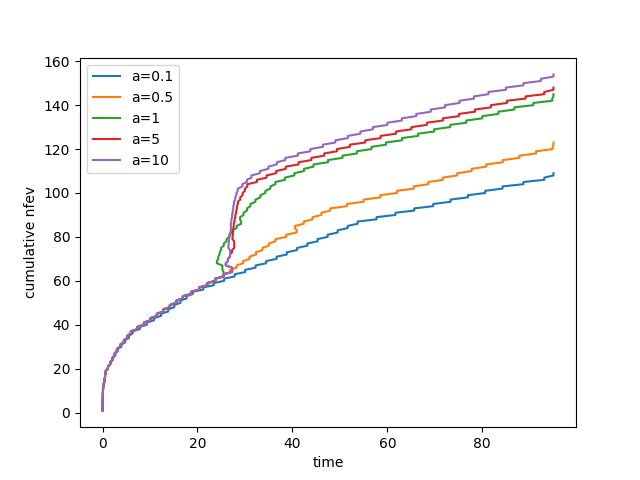
\includegraphics[width=0.7\linewidth]{./figures/exp_thrashing_lsoda}
\caption{Thrashing using the inverse sigmoid to model the change from 0.9 to 0.005 at t=27 with a = 0.1, 0.5, 1, 5, 10 when solving with the LSODA method.}
\label{fig:exp_thrashing_lsoda}
\end{figure}

\begin{figure}[H]
\centering
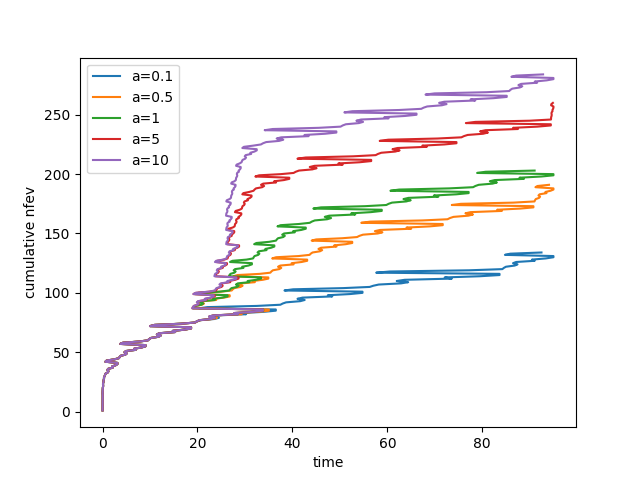
\includegraphics[width=0.7\linewidth]{./figures/exp_thrashing_dop853}
\caption{Thrashing using the inverse sigmoid to model the change from 0.9 to 0.005 at t=27 with a = 0.1, 0.5, 1, 5, 10 when solving with the DOP853 method.}
\label{fig:exp_thrashing_dop853}
\end{figure}

In the remainder of this section, we attempt to solve the time-dependent and state-dependent discontinuity problems with steepness of change, $a$, of 0.1, 1 and 10 to show how using cold starts in the time-dependent discontinuity problem and using event detection in the state-dependent discontinuity problem improves accuracy.

\subsection{Time-dependent discontinuity with exponential change}

\subsubsection{Naive solution of the time-dependent discontinuity with exponential change model}
A naive implementation of the model involves using the inverse sigmoid with $t_c=27$ to model the parameter $\beta$ inside the right-hand side function, $f(t, y)$, to implement the change in $\beta$ as measures are implemented and solving the problem in a single call from $t=0$ to $t=95$. Also, to stay true to a naive treatment, we will use the default tolerances in this section. 

In pseudo code, this looks like:

\begin{minipage}{\linewidth}
\begin{lstlisting}[language=Python]
function model_with_if(t, y)
    // ...
    beta = inverse_sigmoid(t, t_c=27)
    // ...
    // return (dSdt, dEdt, dIdt, dRdt)
\end{lstlisting}
\end{minipage}

Figures $\ref{fig:exp_time_naive_0_1}$, $\ref{fig:exp_time_naive_1}$ and $\ref{fig:exp_time_naive_10}$ shows the naive solution to the time-dependent discontinuity problem using a steepness of change of 0.1, 1 and 10.

\begin{figure}[H]
\centering
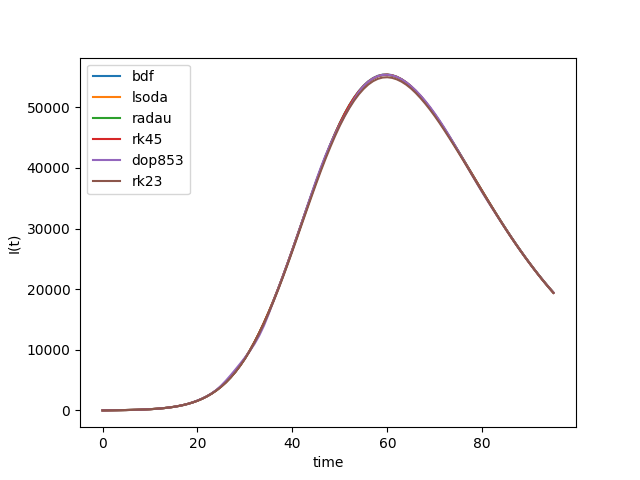
\includegraphics[width=0.7\linewidth]{./figures/exp_time_naive_0_1}
\caption{Naive solution to the time-dependent discontinuity problem with a steepness of change of 0.1.}
\label{fig:exp_time_naive_0_1}
\end{figure}

Figure $\ref{fig:exp_time_naive_0_1}$ shows the naive solution with a steepness of change of 0.1. We can see that the solvers are aligned with each others.

\begin{figure}[H]
\centering
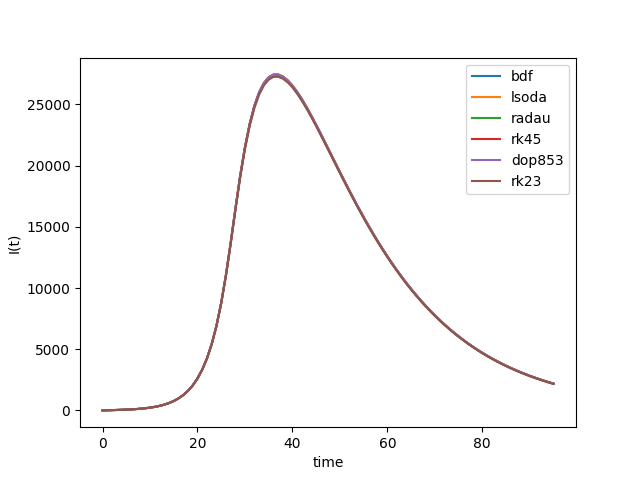
\includegraphics[width=0.7\linewidth]{./figures/exp_time_naive_1}
\caption{Naive solution to the time-dependent discontinuity problem with a steepness of change of 1.}
\label{fig:exp_time_naive_1}
\end{figure}

Figure $\ref{fig:exp_time_naive_1}$ shows the naive solution with a steepness of change of 1. We can see that the solvers are aligned with each others but there is some slight blurring.

\begin{figure}[H]
\centering
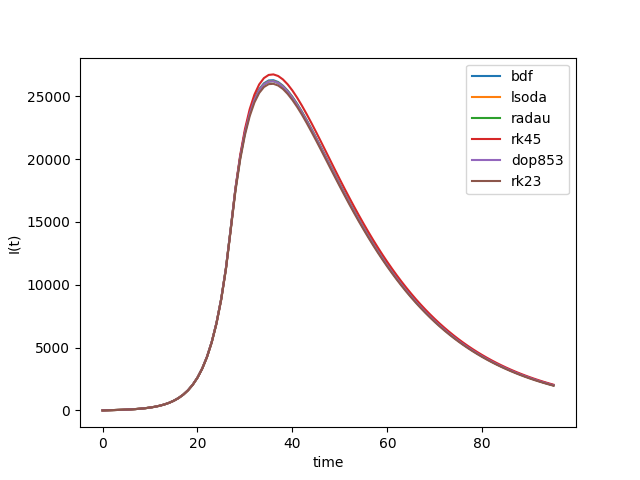
\includegraphics[width=0.7\linewidth]{./figures/exp_time_naive_10}
\caption{Naive solution to the time-dependent discontinuity problem with a steepness of change of 10.}
\label{fig:exp_time_naive_10}
\end{figure}

Figure $\ref{fig:exp_time_naive_10}$ shows the naive solution with a steepness of change of 10. We can see that the solvers are no longer all aligned with each others.

This behaviour is as expected, as the steepness of change grows larger, the problem becomes more discontinuous, there is more thrashing and thus there is a drop in accuracy.

In the next section, we present a solution using cold starts and show how it improves the accuracy.


\subsubsection{Solving the time-dependent discontinuity with exponential change model using a cold start}
As we have seen in the if-statement case, a better way to solve the time-dependent discontinuity problem is to make use of cold starts. This means that we integrate up to the time at which the discontinuity arises and then after the discontinuity we continue the integration with a \emph{separate} call to the solver. 

A cold start means that we restart the solver with method parameters set so that the solver starts the computation with no values from the previous computation. It will also involve using a small initial step size and for methods of varying order like the `BDF' methods, they will restart with the default order which is order 1.

To solve the time dependent discontinuity problem, we will integrate from time 0 to the time that measures are implemented, t=27, with one call to the solver and then use the solution values at t=27 as the initial values to make another call that will integrate (restarting with a cold start) from t=27 to $t_f$. The pseudo-code is as follows:

\begin{minipage}{\linewidth}
\begin{lstlisting}[language=Python]
initial_values = (S0, E0, I0, R0)
tspan_before = [0, 27]
solution_before = ode(intial_values, model_before_measures,
tspan_before)

initial_values_after = extract_last_row(solution_before)
tspan_after = [27, 95]
solution_after = ode(intial_values_after, 
model_after_measures, tspan_after)

solution = concatenate(solution_before, solution_after)
\end{lstlisting}
\end{minipage}

Figures $\ref{fig:exp_time_disc_hand_0_1}$, $\ref{fig:exp_time_disc_hand_1}$ and $\ref{fig:exp_time_disc_hand_10}$ shows the discontinuity handling solutions to the time-dependent discontinuity problem using a steepness of change of 0.1, 1 and 10.

\begin{figure}[H]
\centering
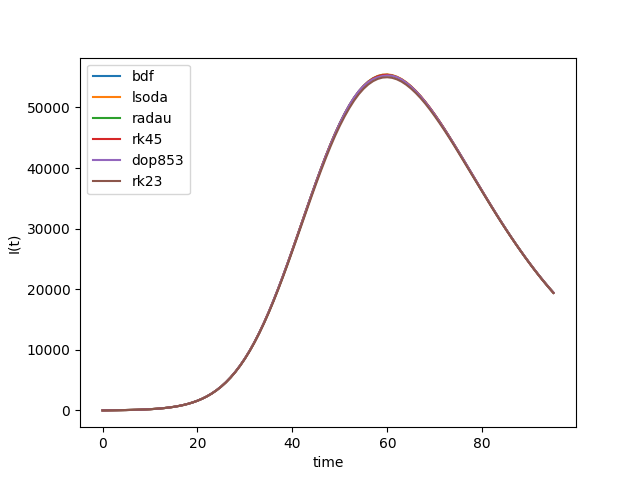
\includegraphics[width=0.7\linewidth]{./figures/exp_time_disc_hand_0_1}
\caption{Solutions to the time-dependent discontinuity model using the inverse sigmoid with a steepness of change of 0.1 using solvers from Python and a cold start at t=27.}
\label{fig:exp_time_disc_hand_0_1}
\end{figure}

\begin{figure}[H]
\centering
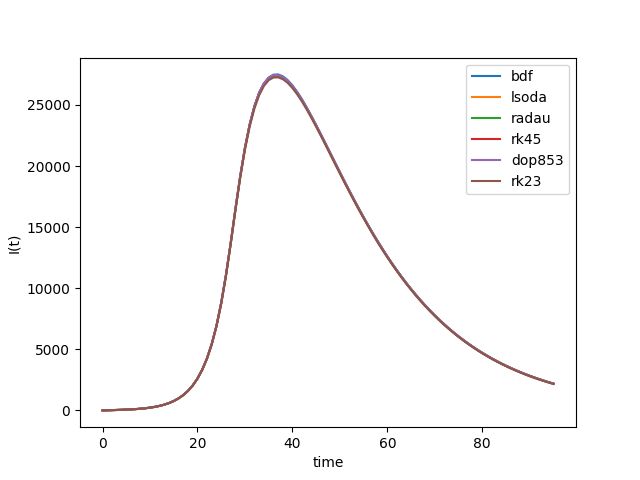
\includegraphics[width=0.7\linewidth]{./figures/exp_time_disc_hand_1}
\caption{Solutions to the time-dependent discontinuity model using the inverse sigmoid with a steepness of change of 1 using solvers from Python and a cold start at t=27.}
\label{fig:exp_time_disc_hand_1}
\end{figure}

\begin{figure}[H]
\centering
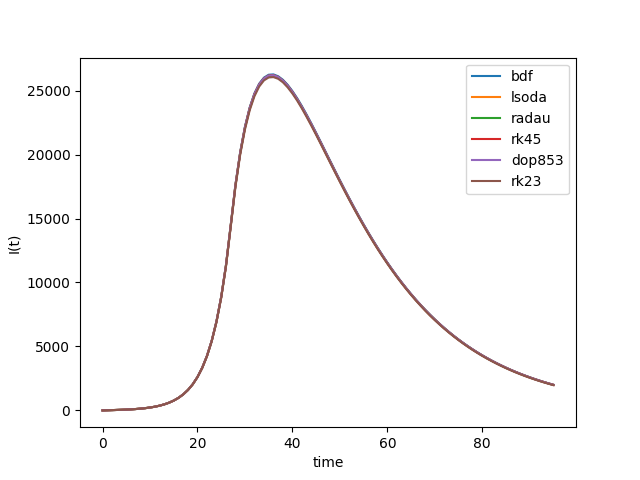
\includegraphics[width=0.7\linewidth]{./figures/exp_time_disc_hand_10}
\caption{Solutions to the time-dependent discontinuity model using the inverse sigmoid with a steepness of change of 10 using solvers from Python and a cold start at t=27.}
\label{fig:exp_time_disc_hand_10}
\end{figure}

Using the cold state at $t=27$ allowed the solvers to produce solutions that are aligned at all three different steepness of change. Thus the cold start improved accuracy.

However the efficiency of the solvers is not improved by much.

\begin{table}[H]
\caption {Python efficiency data for the time-dependent discontinuity problem with a steepness of change of 0.1 - number of function evaluations} 
\label{tab:exp_time_0_1} 
\begin{center}
\begin{tabular}{ c c c }
method & no discontinuity handling & with discontinuity handling \\ 
lsoda & 109 & 116 \\
rk45 & 116 & 130 \\
bdf & 127 & 140 \\
radau & 182 & 201 \\
dop853 & 134 & 181 \\
rk23 & 113 & 121 \\
\end{tabular}
\end{center}
\end{table}

\begin{table}[H]
\caption {Python efficiency data for the time-dependent discontinuity problem with a steepness of change of 1 - number of function evaluations} 
\label{tab:exp_time_1} 
\begin{center}
\begin{tabular}{ c c c }
method & no discontinuity handling & with discontinuity handling \\ 
lsoda & 145 & 150 \\
rk45 & 122 & 136 \\
bdf & 166 & 173 \\
radau & 241 & 247 \\
dop853 & 203 & 211 \\
rk23 & 131 & 139 \\
\end{tabular}
\end{center}
\end{table}

\begin{table}[H]
\caption {Python efficiency data for the time-dependent discontinuity problem with a steepness of change of 10 - number of function evaluations} 
\label{tab:exp_time_10} 
\begin{center}
\begin{tabular}{ c c c }
method & no discontinuity handling & with discontinuity handling \\ 
lsoda & 154 & 164 \\
rk45 & 140 & 148 \\
bdf & 186 & 174 \\
radau & 288 & 287 \\
dop853 & 284 & 262 \\
rk23 & 134 & 142 \\
\end{tabular}
\end{center}
\end{table}

\subsubsection{LSODA time-dependent discontinuity with exponential change problem tolerance study}
\paragraph{steepness of change of 0.1}

\begin{figure}[H]
\centering
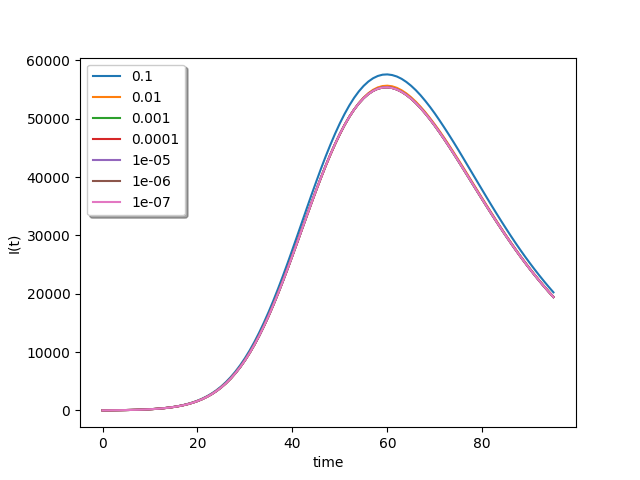
\includegraphics[width=0.7\linewidth]{./figures/exp_time_tol_lsoda_no_event_0_1}
\caption{Time-dependent discontinuity model tolerance study on the Python version of LSODA without a cold start with a steepness of change of 0.1.}
\label{fig:exp_time_tol_lsoda_no_event_0_1}
\end{figure}

\begin{figure}[H]
\centering
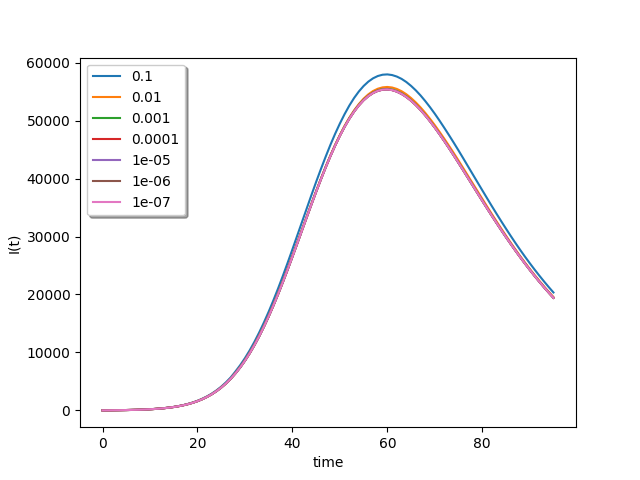
\includegraphics[width=0.7\linewidth]{./figures/exp_time_tol_lsoda_event_0_1}
\caption{Time-dependent discontinuity model tolerance study on the Python version of LSODA with a cold start with a steepness of change of 0.1.}
\label{fig:exp_time_tol_lsoda_event_0_1}
\end{figure}

\begin{table}[H]
\caption {Python LSODA time-dependent discontinuity model with exponential change with a steepness of change of 0.1 tolerance study - number of function evaluations} \label{tab:exp_time_tol_lsoda_0_1} 
\begin{center}
\begin{tabular}{ c c c }
tolerance & no discontinuity handling & with discontinuity handling \\ 
0.1 & 78.0 & 87.0 \\
0.01 & 81.0 & 93.0 \\
0.001 & 99.0 & 108.0 \\
0.0001 & 127.0 & 136.0 \\
1e-05 & 161.0 & 176.0 \\
1e-06 & 199.0 & 228.0 \\
1e-07 & 235.0 & 266.0 \\
\end{tabular}
\end{center}
\end{table}

\paragraph{steepness of change of 1}

\begin{figure}[H]
\centering
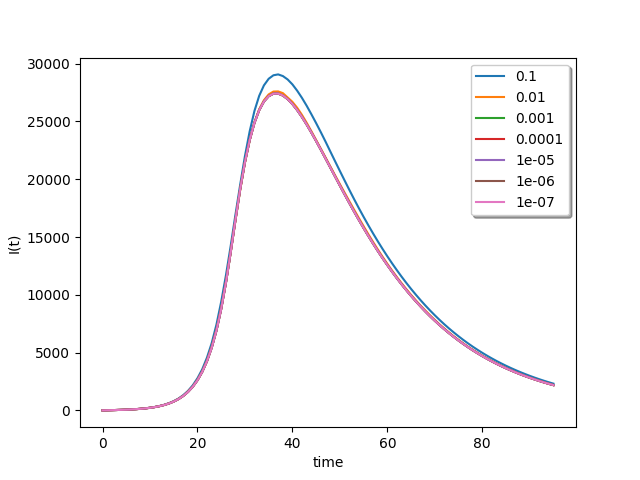
\includegraphics[width=0.7\linewidth]{./figures/exp_time_tol_lsoda_no_event_1}
\caption{Time-dependent discontinuity model tolerance study on the Python version of LSODA without a cold start with a steepness of change of 1.}
\label{fig:exp_time_tol_lsoda_no_event_1}
\end{figure}

\begin{figure}[H]
\centering
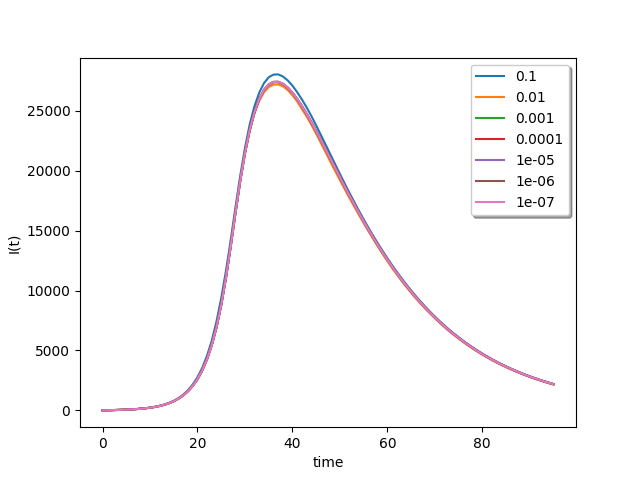
\includegraphics[width=0.7\linewidth]{./figures/exp_time_tol_lsoda_event_1}
\caption{Time-dependent discontinuity model tolerance study on the Python version of LSODA with a cold start with a steepness of change of 1.}
\label{fig:exp_time_tol_lsoda_event_1}
\end{figure}

\begin{table}[H]
\caption {Python LSODA time-dependent discontinuity model with exponential change with a steepness of change of 1 tolerance study - number of function evaluations} \label{tab:exp_time_tol_lsoda_1} 
\begin{center}
\begin{tabular}{ c c c }
tolerance & no discontinuity handling & with discontinuity handling \\ 
0.1 & 78.0 & 88.0 \\
0.01 & 89.0 & 99.0 \\
0.001 & 135.0 & 140.0 \\
0.0001 & 173.0 & 182.0 \\
1e-05 & 215.0 & 234.0 \\
1e-06 & 261.0 & 286.0 \\
1e-07 & 333.0 & 370.0 \\
\end{tabular}
\end{center}
\end{table}


\paragraph{steepness of change of 10}

\begin{figure}[H]
\centering
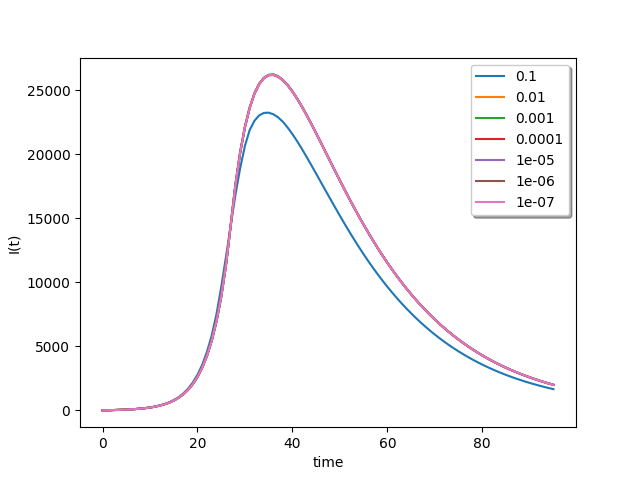
\includegraphics[width=0.7\linewidth]{./figures/exp_time_tol_lsoda_no_event_10}
\caption{Time-dependent discontinuity model tolerance study on the Python version of LSODA without a cold start with a steepness of change of 10.}
\label{fig:exp_time_tol_lsoda_no_event_10}
\end{figure}

\begin{figure}[H]
\centering
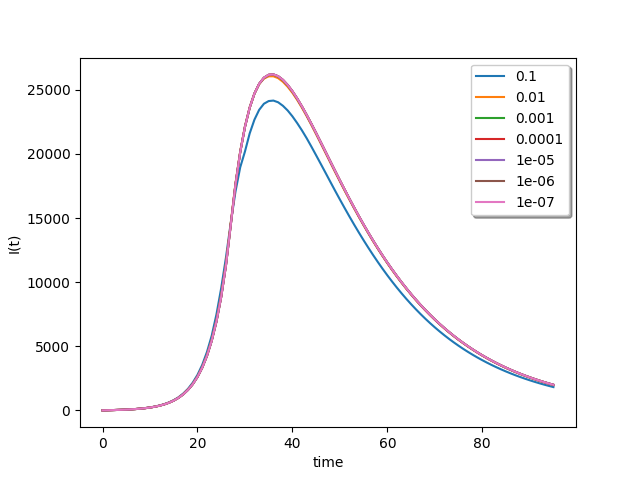
\includegraphics[width=0.7\linewidth]{./figures/exp_time_tol_lsoda_event_10}
\caption{Time-dependent discontinuity model tolerance study on the Python version of LSODA with a cold start with a steepness of change of 10.}
\label{fig:exp_time_tol_lsoda_event_10}
\end{figure}

\begin{table}[H]
\caption {Python LSODA time-dependent discontinuity model with exponential change with a steepness of change of 1 tolerance study - number of function evaluations} \label{tab:exp_time_tol_lsoda_10} 
\begin{center}
\begin{tabular}{ c c c }
tolerance & no discontinuity handling & with discontinuity handling \\ 
0.1 & 77.0 & 86.0 \\
0.01 & 98.0 & 99.0 \\
0.001 & 140.0 & 151.0 \\
0.0001 & 191.0 & 205.0 \\
1e-05 & 264.0 & 263.0 \\
1e-06 & 320.0 & 335.0 \\
1e-07 & 386.0 & 415.0 \\
\end{tabular}
\end{center}
\end{table}


\subsubsection{RK45 time-dependent discontinuity problem tolerance study}
\paragraph{steepness of change of 0.1}

\begin{figure}[H]
\centering
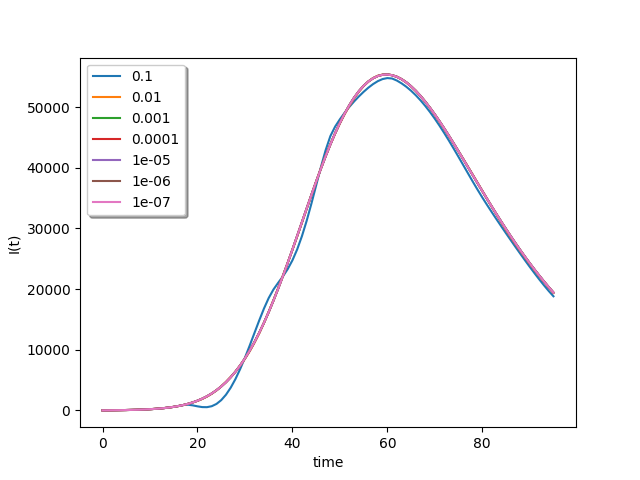
\includegraphics[width=0.7\linewidth]{./figures/exp_time_tol_rk45_no_event_0_1}
\caption{Time-dependent discontinuity model tolerance study on the Python version of RK45 without a cold start with a steepness of change of 0.1.}
\label{fig:exp_time_tol_rk45_no_event_0_1}
\end{figure}

\begin{figure}[H]
\centering
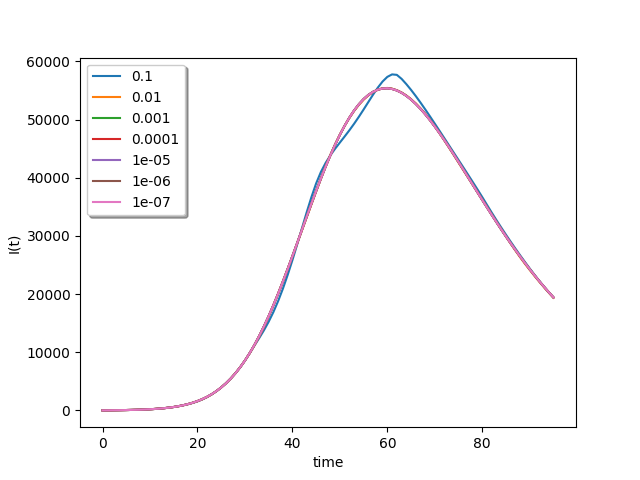
\includegraphics[width=0.7\linewidth]{./figures/exp_time_tol_rk45_event_0_1}
\caption{Time-dependent discontinuity model tolerance study on the Python version of RK45 with a cold start with a steepness of change of 0.1.}
\label{fig:exp_time_tol_rk45_event_0_1}
\end{figure}

\begin{table}[H]
\caption {Python RK45 time-dependent discontinuity model with exponential change with a steepness of change of 0.1 tolerance study - number of function evaluations} \label{tab:exp_time_tol_rk45_0_1} 
\begin{center}
\begin{tabular}{ c c c }
tolerance & no discontinuity handling & with discontinuity handling \\ 
0.1 & 62.0 & 70.0 \\
0.01 & 80.0 & 94.0 \\
0.001 & 110.0 & 130.0 \\
0.0001 & 158.0 & 172.0 \\
1e-05 & 230.0 & 244.0 \\
1e-06 & 350.0 & 370.0 \\
1e-07 & 536.0 & 550.0 \\
\end{tabular}
\end{center}
\end{table}

\paragraph{steepness of change of 1}

\begin{figure}[H]
\centering
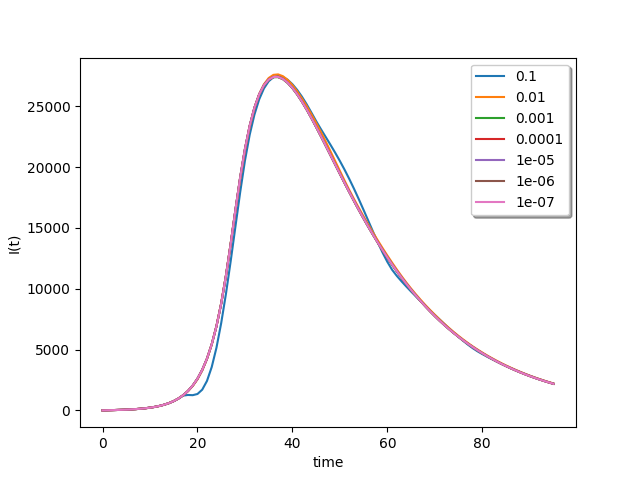
\includegraphics[width=0.7\linewidth]{./figures/exp_time_tol_rk45_no_event_1}
\caption{Time-dependent discontinuity model tolerance study on the Python version of RK45 without a cold start with a steepness of change of 1.}
\label{fig:exp_time_tol_rk45_no_event_1}
\end{figure}

\begin{figure}[H]
\centering
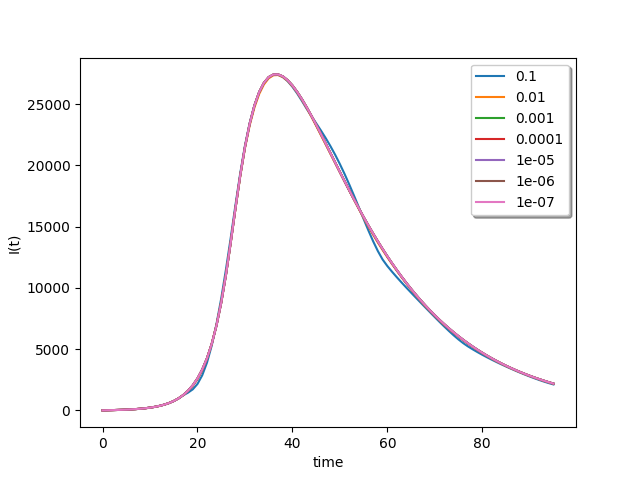
\includegraphics[width=0.7\linewidth]{./figures/exp_time_tol_rk45_event_1}
\caption{Time-dependent discontinuity model tolerance study on the Python version of RK45 with a cold start with a steepness of change of 1.}
\label{fig:exp_time_tol_rk45_event_1}
\end{figure}

\begin{table}[H]
\caption {Python RK45 time-dependent discontinuity model with exponential change with a steepness of change of 1 tolerance study - number of function evaluations} \label{tab:exp_time_tol_rk45_1} 
\begin{center}
\begin{tabular}{ c c c }
tolerance & no discontinuity handling & with discontinuity handling \\ 
0.1 & 68.0 & 76.0 \\
0.01 & 86.0 & 100.0 \\
0.001 & 116.0 & 130.0 \\
0.0001 & 164.0 & 178.0 \\
1e-05 & 248.0 & 262.0 \\
1e-06 & 374.0 & 382.0 \\
1e-07 & 572.0 & 586.0 \\
\end{tabular}
\end{center}
\end{table}


\paragraph{steepness of change of 10}

\begin{figure}[H]
\centering
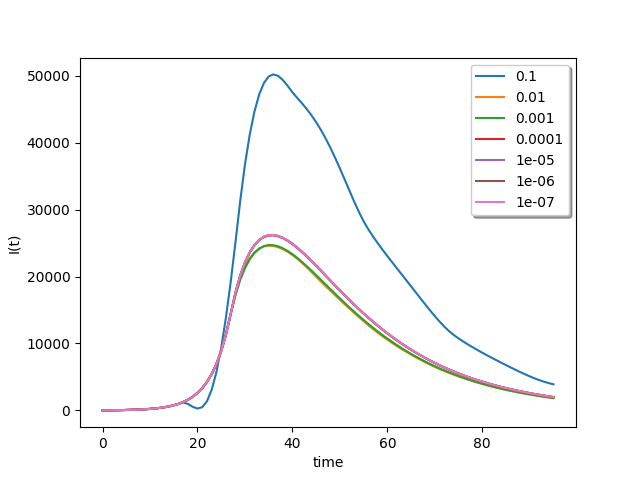
\includegraphics[width=0.7\linewidth]{./figures/exp_time_tol_rk45_no_event_10}
\caption{Time-dependent discontinuity model tolerance study on the Python version of RK45 without a cold start with a steepness of change of 10.}
\label{fig:exp_time_tol_rk45_no_event_10}
\end{figure}

\begin{figure}[H]
\centering
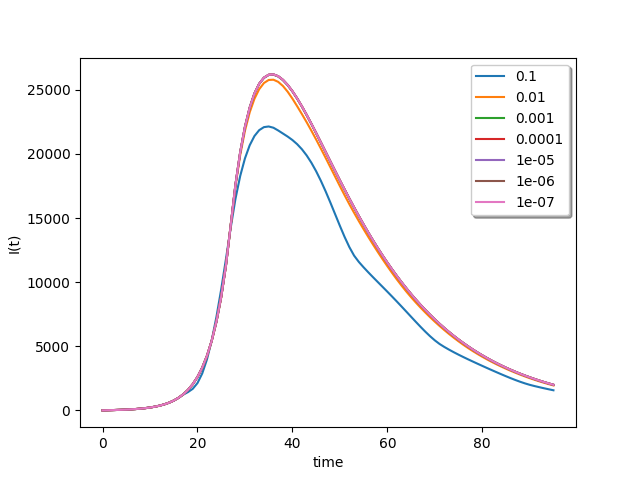
\includegraphics[width=0.7\linewidth]{./figures/exp_time_tol_rk45_event_10}
\caption{Time-dependent discontinuity model tolerance study on the Python version of RK45 with a cold start with a steepness of change of 10.}
\label{fig:exp_time_tol_rk45_event_10}
\end{figure}

\begin{table}[H]
\caption {Python RK45 time-dependent discontinuity model with exponential change with a steepness of change of 1 tolerance study - number of function evaluations} \label{tab:exp_time_tol_rk45_10} 
\begin{center}
\begin{tabular}{ c c c }
tolerance & no discontinuity handling & with discontinuity handling \\ 
0.1 & 68.0 & 76.0 \\
0.01 & 86.0 & 106.0 \\
0.001 & 116.0 & 124.0 \\
0.0001 & 182.0 & 190.0 \\
1e-05 & 284.0 & 292.0 \\
1e-06 & 410.0 & 424.0 \\
1e-07 & 644.0 & 652.0 \\
\end{tabular}
\end{center}
\end{table}


\subsection{State-dependent discontinuity with exponential change}
In this section, we consider an extension of the state-dependent discontinuity problem where we use the sigmoid and inverse sigmoid function to change the parameter $\beta$ instead of if-statements. We again attempt a long term forecast where measures are introduced and relaxed based on E(t), the number of exposed individuals at time, t.



As in Section $\ref{section:time_problem}$, changes in the modelling parameter $\beta$ introduce discontinuities in the function $f(t, y(t))$ and thus the error control solvers will ``thrash" when trying to solve the problem (as described in Section $\ref{subsection:effect_of_discontinuity}$). 
%We will show that the presence of several discontinuities makes the problem challenging enough that all the ODE solvers we consider, even at very sharp tolerances, will not be able to solve the problem with reasonable accuracy.

When there are no measures and E(t) crosses 25000, we assume that measures are introduced which will reduce the value of the parameter $\beta$ from 0.9 to 0.005. When there are no measures and E(t) crosses 10000, we assume that measures are relaxed which increases the value of the parameter $\beta$ from 0.005 back to 0.9.

We start with a simple treatment of the problem with `if' statements employed inside the function that defines the right-hand side of the ODE system which choses between the sigmoid and the inverse sigmoid centered at the time of the last change based on whether measures are introduced or not and show how this form of the problem cannot be solved with reasonable accuracy, by any of the solvers, even at sharp tolerances. Finally, we will introduce an approach to efficiently and accurately solve the problem using an approach involving the use of what is known as event detection to handle the discontinuities.
\subsubsection{Naive solution of the state-dependent discontinuity with exponential change model}
A simple treatment of this problem is to use global variables for tracking when measures are implemented and relaxed and to toggle these global variables as we reach the required thresholds. We use this approach because we need to know if the number of exposed people is going up or down to know whether we need to check for the maximum or the minimum threshold. We then have an `if' statement that will choose between the sigmoid and inverse sigmoid function centered at the time of the last change, also a global variable, for the parameter $\beta$ based on whether measures are being implemented or not. The pseudo-code for this algorithm is as follows:

\begin{minipage}{\linewidth}
\begin{lstlisting}[language=Python]
measures_implemented = False
direction = "up"
time_last_changed = 0

function model_with_if(t, y):
    // ...
    global measures_implemented, direction, time_last_changed
    if (direction == "up"):
        if (E > 25000):
            measures_implemented = True
            direction = "down"
            time_last_changed = t
    else:
        if (E < 10000):
            measures_implemented = False
            direction = "up"
            time_last_changed = t

    if measures_implemented:
        beta = inverse_sigmoid(t, t_c=time_last_changed)
    else:
        beta = sigmoid(t, t_c=time_last_changed)
    // ...
    return (dSdt, dEdt, dIdt, dRdt)
\end{lstlisting}
\end{minipage}

Figures $\ref{fig:exp_state_naive_0_1}$, $\ref{fig:exp_state_naive_1}$ and $\ref{fig:exp_state_naive_10}$ shows the naive solution to the state-dependent discontinuity problem using a steepness of change of 0.1, 1 and 10.

\begin{figure}[H]
\centering
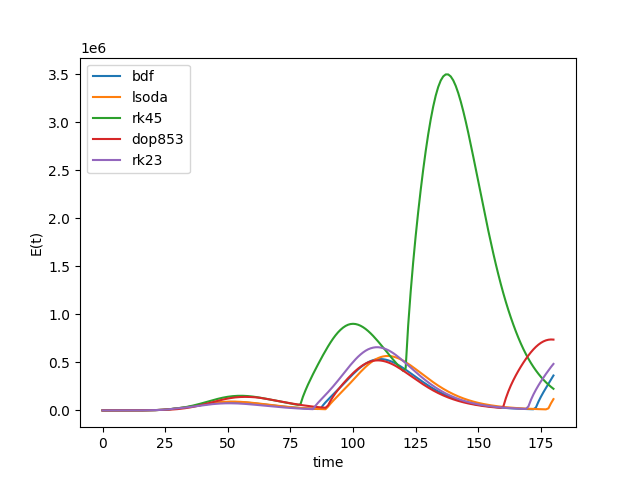
\includegraphics[width=0.7\linewidth]{./figures/exp_state_naive_0_1}
\caption{Naive solution to the state-dependent discontinuity problem with a steepness of change of 0.1.}
\label{fig:exp_state_naive_0_1}
\end{figure}

\begin{figure}[H]
\centering
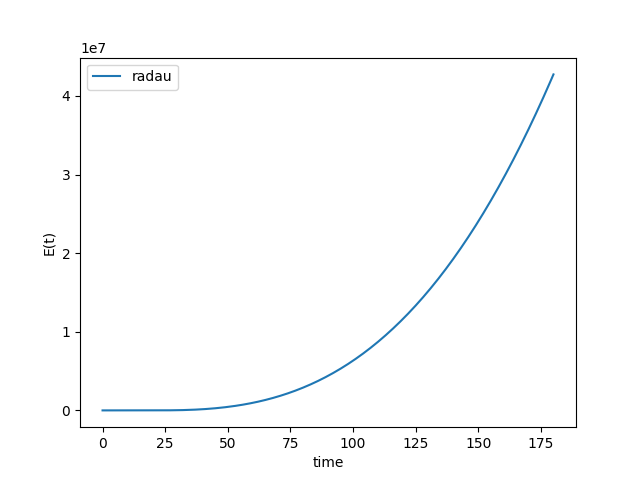
\includegraphics[width=0.7\linewidth]{./figures/exp_state_naive_radau_0_1}
\caption{Naive solution computed by `Radau' to the state-dependent discontinuity problem with a steepness of change of 0.1.}
\label{fig:exp_state_naive_radau_0_1}
\end{figure}

\begin{figure}[H]
\centering
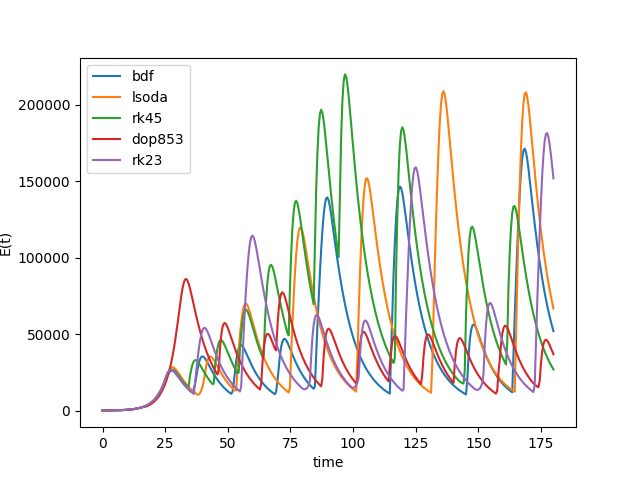
\includegraphics[width=0.7\linewidth]{./figures/exp_state_naive_1}
\caption{Naive solution to the state-dependent discontinuity problem with a steepness of change of 1.}
\label{fig:exp_state_naive_1}
\end{figure}

\begin{figure}[H]
\centering
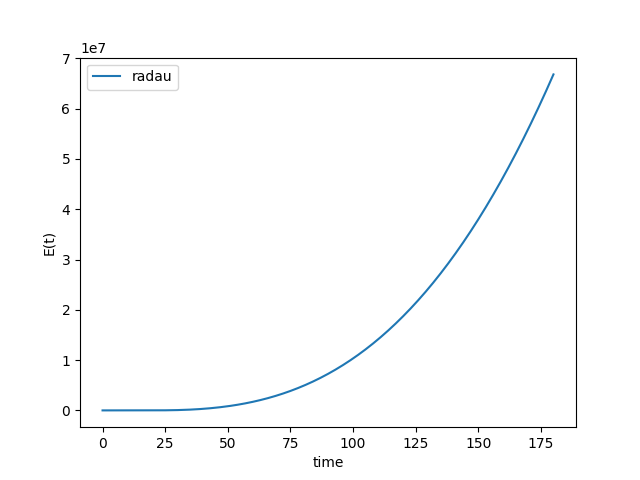
\includegraphics[width=0.7\linewidth]{./figures/exp_state_naive_radau_1}
\caption{Naive solution computed by `Radau' to the state-dependent discontinuity problem with a steepness of change of 1.}
\label{fig:exp_state_naive_radau_1}
\end{figure}


\begin{figure}[H]
\centering
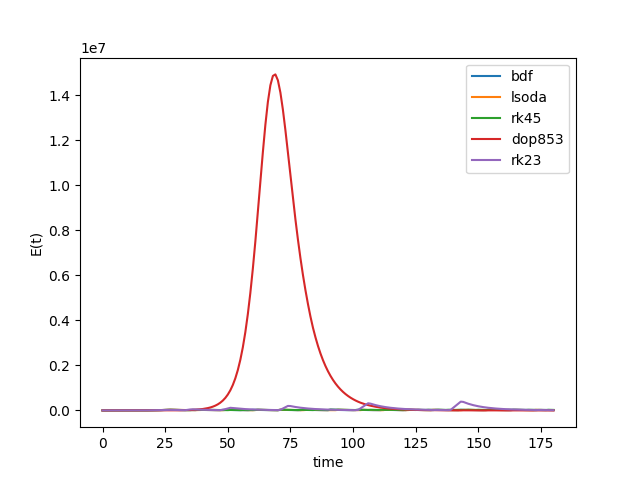
\includegraphics[width=0.7\linewidth]{./figures/exp_state_naive_10}
\caption{Naive solution to the state-dependent discontinuity problem with a steepness of change of 10.}
\label{fig:exp_state_naive_10}
\end{figure}

\begin{figure}[H]
\centering
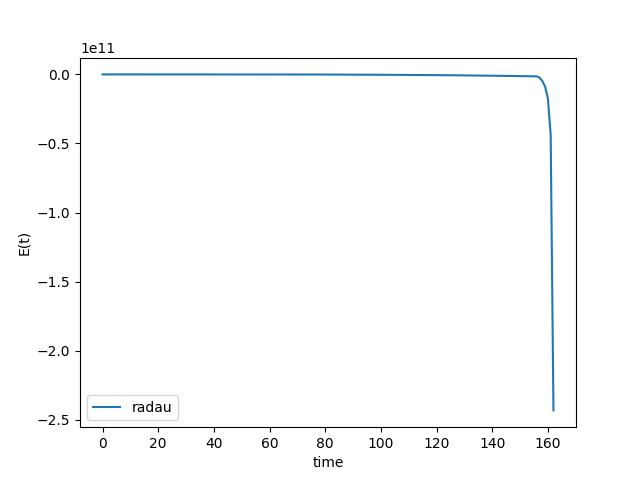
\includegraphics[width=0.7\linewidth]{./figures/exp_state_naive_radau_10}
\caption{Naive solution computed by `Radau' to the state-dependent discontinuity problem with a steepness of change of 10.}
\label{fig:exp_state_naive_radau_10}
\end{figure}

\subsubsection{Naive sharp tolerance solution of the state-dependent discontinuity with exponential change model}

Figures $\ref{fig:exp_state_naive_sharp_0_1}$, $\ref{fig:exp_state_naive_sharp_1}$ and $\ref{fig:exp_state_naive_sharp_10}$ shows the naive solution to the state-dependent discontinuity problem using a steepness of change of 0.1, 1 and 10 at an absolute tolerance of $10^{-12}$ and a relative tolerance of $10^{-12}$.

\begin{figure}[H]
\centering
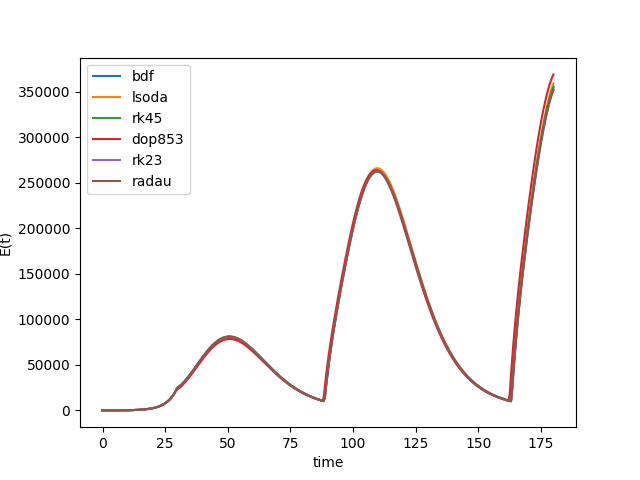
\includegraphics[width=0.7\linewidth]{./figures/exp_state_naive_sharp_0_1}
\caption{Naive sharp tolerance solution to the state-dependent discontinuity problem with a steepness of change of 0.1.}
\label{fig:exp_state_naive_sharp_0_1}
\end{figure}


\begin{figure}[H]
\centering
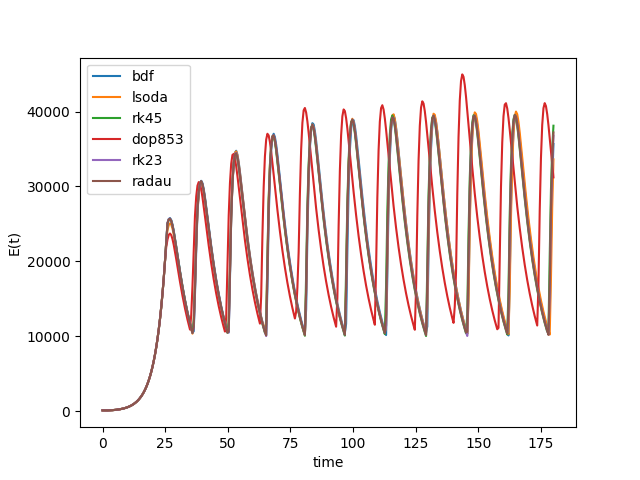
\includegraphics[width=0.7\linewidth]{./figures/exp_state_naive_sharp_1}
\caption{Naive sharp tolerance solution to the state-dependent discontinuity problem with a steepness of change of 1.}
\label{fig:exp_state_naive_sharp_1}
\end{figure}

\begin{figure}[H]
\centering
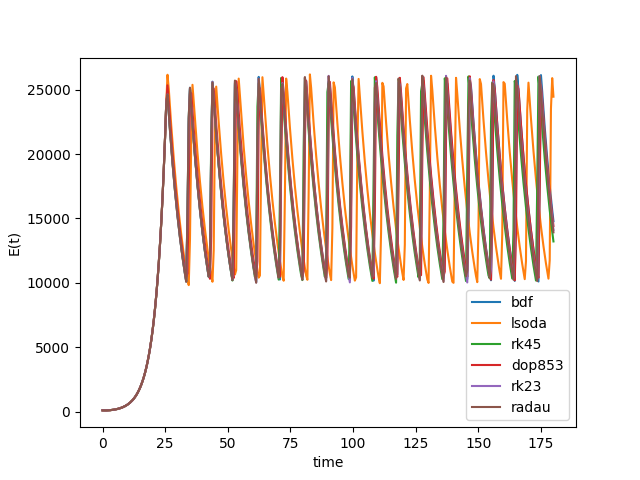
\includegraphics[width=0.7\linewidth]{./figures/exp_state_naive_sharp_10}
\caption{Naive sharp tolerance solution to the state-dependent discontinuity problem with a steepness of change of 10.}
\label{fig:exp_state_naive_sharp_10}
\end{figure}


\subsubsection{Solving the state-dependent discontinuity with exponential change model using event detection}
We can see that with this version of the state-dependent discontinuity problem, using a sharp tolerance allows us to get solutions that are aligned with each others. We then use event detection to try to see if we can get more accurate solutions.

Again we use the idea of defining the thresholds as events. When an event is detected, that is a threshold is crossed, we cold start the solver with a new right hand side function using either the sigmoid or inverse sigmoid function centered at the time of the last event for the value of the $\beta$ parameter and a new root function. 

For our specific problem, event detection is used as follows.
We start by solving the problem with $\beta$ using sigmoid function growing from 0.005 to 0.9 centered at $t-0$ and with a root function that detects when E(t) is equal to 25000. Once, using the event detection capability of the solver, we reach the time at which $E(t)=25000$, we do a cold start. We evaluate the solution computed by the solver at the time of the event and use that solution as the initial value for our next call to the solver. This next call will have $\beta$ using the inverse sigmoid function decreasing from 0.9 to 0.005 centered at the time of the $E(t)=25000$ event just recorded and a root function that detects a root when $E(t)=10000$. We again integrate up to that new threshold and cold start when we reach it. The new integration will have $\beta$ using the sigmoid function growing from 0.005 to 0.9 centered at the time of the $E(t)=10000$ event just recorded and the root function will look for $E(t)=25000$ as the event. This is repeated until we reach the desired end time. The pseudo-code is as follows:

\begin{minipage}{\linewidth}
\centering
\begin{lstlisting}[language=Python]
function model_no_measures(t, y, time_last_event):
    beta = sigmoid(t, t_c=time_last_event)
    // code to get dSdt, dEdt, dIdt, dRdt
    return (dSdt, dEdt, dIdt, dRdt)

function root_25000(t, y):
    E = y[1]
    return E - 25000

function model_with_measures(t, y, time_last_event):
    beta = inverse_sigmoid(t, t_c=time_last_event)
    // code to get dSdt, dEdt, dIdt, dRdt
    return (dSdt, dEdt, dIdt, dRdt)

function root_10000(t, y):
    E = y[1]
    return E - 10000

res = array()
t_initial = 0
y_initial = (S0, E0, I0, R0)
while t_initial < 180:
    tspan = [t_initial, 180]
    if (measures_implemented):
        sol = ode(model_with_measures, tspan, y_initial,
            events=root_10000, args=[t_initial])
        measures_implemented = False
    else:
        sol = ode(model_no_measures, tspan, y_initial,
            events=root_25000, args=[t_initial])
        measures_implemented = True
    t_initial = extract_last_t_from_sol(sol)
    y_initial = extract_last_row_from_sol(sol)
    res = concatenate(res, sol)

// use res as the final solution
\end{lstlisting}
\end{minipage}

Figures $\ref{fig:exp_state_event_0_1}$, $\ref{fig:exp_state_event_1}$ and $\ref{fig:exp_state_event_10}$ shows the solution using event detection to the state-dependent discontinuity problem using a steepness of change of 0.1, 1 and 10.

\begin{figure}[H]
\centering
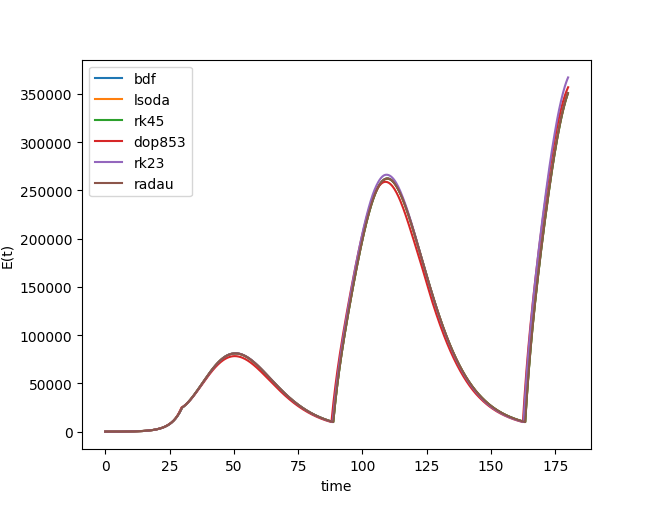
\includegraphics[width=0.7\linewidth]{./figures/exp_state_event_0_1}
\caption{Solution using event detection to the state-dependent discontinuity problem with a steepness of change of 0.1.}
\label{fig:exp_state_event_0_1}
\end{figure}

\begin{table}[h]
\caption {Efficiency data for Python state-dependent discontinuity model with exponential change with a steepness of change of 0.1 - number of function evaluations} \label{tab:exp_state_0_1}
\begin{center}
\begin{tabular}{ c c c c } 
method & no event & no event with sharp tol. & with event detection \\ 
lsoda & 296   & 1389   & 240 \\
bdf & 393     & 5663   & 297 \\
radau & 204   & 48529  & 397 \\
rk45 & 272    & 10136  & 282 \\
dop853 & 1094 & 4817   & 432 \\
rk23 & 293    & 168026 & 237 \\
\end{tabular}
\end{center}
\end{table}

\begin{figure}[H]
\centering
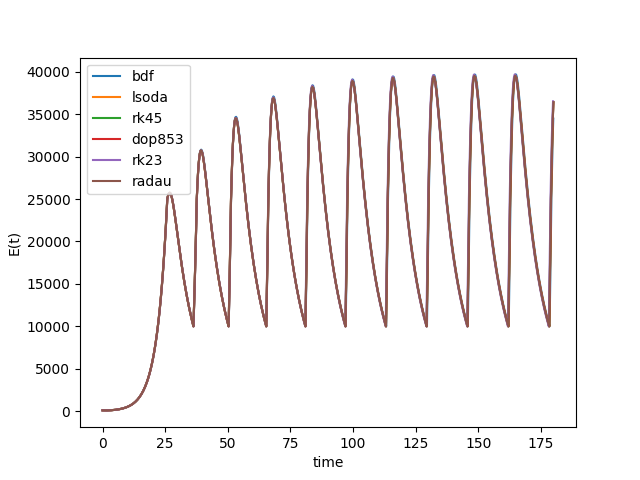
\includegraphics[width=0.7\linewidth]{./figures/exp_state_event_1}
\caption{Solution using event detection to the state-dependent discontinuity problem with a steepness of change of 1.}
\label{fig:exp_state_event_1}
\end{figure}

\begin{table}[h]
\caption {Efficiency data for Python state-dependent discontinuity model with exponential change with a steepness of change of 1 - number of function evaluations} \label{tab:exp_state_1}
\begin{center}
\begin{tabular}{ c c c c } 
method & no event & no event with sharp tol. & with event detection \\ 
lsoda & 589   & 4829    & 548 \\
bdf & 811     & 14642   & 758 \\
radau & 211   & 96933   & 1076 \\
rk45 & 566    & 15800   & 584 \\
dop853 & 2648 & 14558   & 1184 \\
rk23 & 653    & 306788  & 527 \\
\end{tabular}
\end{center}
\end{table}


\begin{figure}[H]
\centering
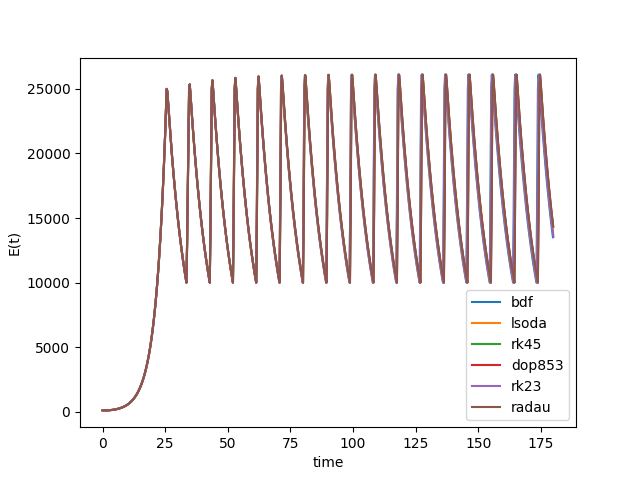
\includegraphics[width=0.7\linewidth]{./figures/exp_state_event_10}
\caption{Solution using event detection to the state-dependent discontinuity problem with a steepness of change of 10.}
\label{fig:exp_state_event_10}
\end{figure}

\begin{table}[h]
\caption {Efficiency data for Python state-dependent discontinuity model with exponential change with a steepness of change of 10 - number of function evaluations} \label{tab:exp_state_10}
\begin{center}
\begin{tabular}{ c c c c } 
method & no event & no event with sharp tol. & with event detection \\ 
lsoda & 1503   & 11518    & 1098 \\
bdf & 1235     & 27795    & 1192 \\
radau & 1810   & 164687   & 1739 \\
rk45 & 2384    & 25994    & 842 \\
dop853 & 992   & 27092    & 2063 \\
rk23 & 572     & 440066   & 785 \\

\end{tabular}
\end{center}
\end{table}

\subsubsection{LSODA state-dependent discontinuity problem tolerance study}
\paragraph{steepness of change of 0.1}

\begin{figure}[H]
\centering
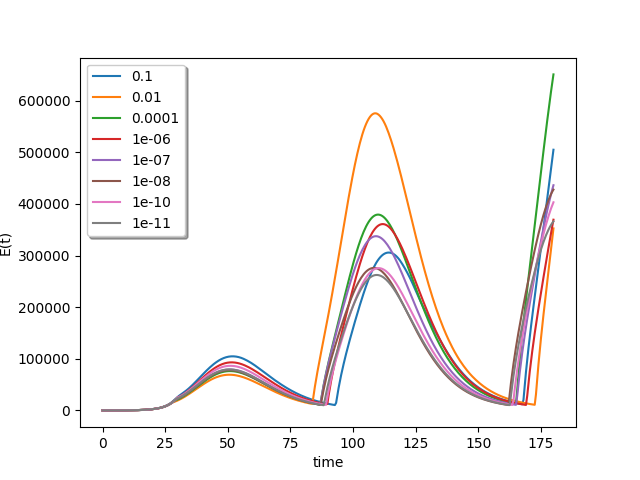
\includegraphics[width=0.7\linewidth]{./figures/exp_state_tol_lsoda_no_event_0_1}
\caption{State-dependent discontinuity model tolerance study on the Python version of LSODA without event detection with a steepness of change of 0.1.}
\label{fig:exp_state_tol_lsoda_no_event_0_1}
\end{figure}

\begin{figure}[H]
\centering
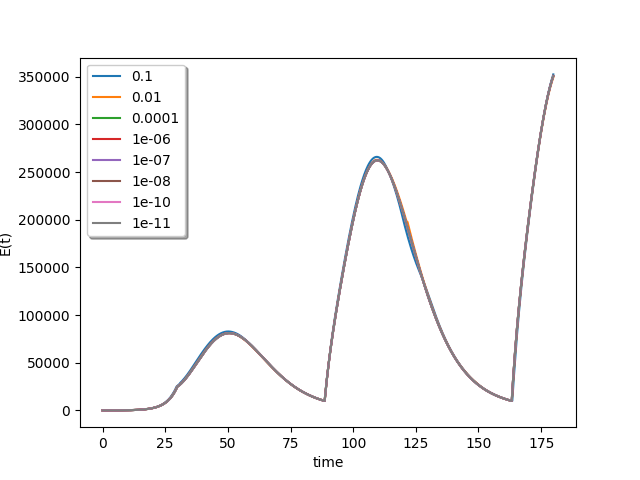
\includegraphics[width=0.7\linewidth]{./figures/exp_state_tol_lsoda_event_0_1}
\caption{State-dependent discontinuity model tolerance study on the Python version of LSODA with event detection with a steepness of change of 0.1.}
\label{fig:exp_state_tol_lsoda_event_0_1}
\end{figure}

\begin{table}[H]
\caption {Python LSODA state-dependent discontinuity model with exponential change with a steepness of change of 0.1 tolerance study - number of function evaluations} \label{tab:exp_state_tol_lsoda_0_1} 
\begin{center}
\begin{tabular}{ c c c }
tolerance & no event detection & with event detection \\ 
0.1 & 200 & 182 \\
0.01 & 246 & 192 \\
0.0001 & 345 & 300 \\
1e-06 & 515 & 478 \\
1e-07 & 621 & 620 \\
1e-08 & 782 & 738 \\
1e-10 & 993 & 980 \\
1e-11 & 1200 & 1127 \\
\end{tabular}
\end{center}
\end{table}

\paragraph{steepness of change of 1}
\begin{figure}[H]
\centering
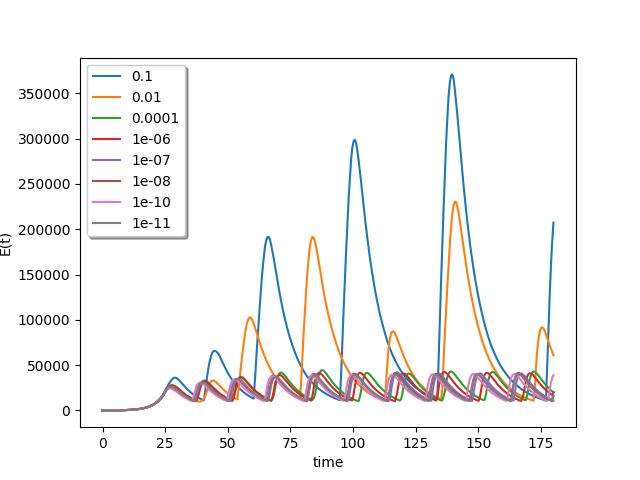
\includegraphics[width=0.7\linewidth]{./figures/exp_state_tol_lsoda_no_event_1}
\caption{State-dependent discontinuity model tolerance study on the Python version of LSODA without event detection with a steepness of change of 1.}
\label{fig:exp_state_tol_lsoda_no_event_1}
\end{figure}

\begin{figure}[H]
\centering
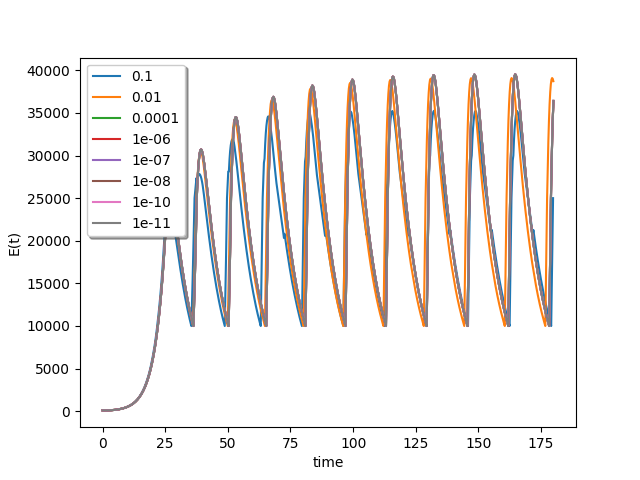
\includegraphics[width=0.7\linewidth]{./figures/exp_state_tol_lsoda_event_1}
\caption{State-dependent discontinuity model tolerance study on the Python version of LSODA with event detection with a steepness of change of 1.}
\label{fig:exp_state_tol_lsoda_event_1}
\end{figure}

\begin{table}[H]
\caption {Python LSODA state-dependent discontinuity model with exponential change with a steepness of change of 1 tolerance study - number of function evaluations} \label{tab:exp_state_tol_lsoda_1} 
\begin{center}
\begin{tabular}{ c c c }
tolerance & no event detection & with event detection \\ 
0.1 & 339 & 353 \\
0.01 & 437 & 431 \\
0.0001 & 1133 & 786 \\
1e-06 & 1793 & 1406 \\
1e-07 & 2170 & 1748 \\
1e-08 & 2640 & 2242 \\
1e-10 & 3559 & 3271 \\
1e-11 & 4059 & 3707 \\
\end{tabular}
\end{center}
\end{table}



\paragraph{steepness of change of 10}
\begin{figure}[H]
\centering
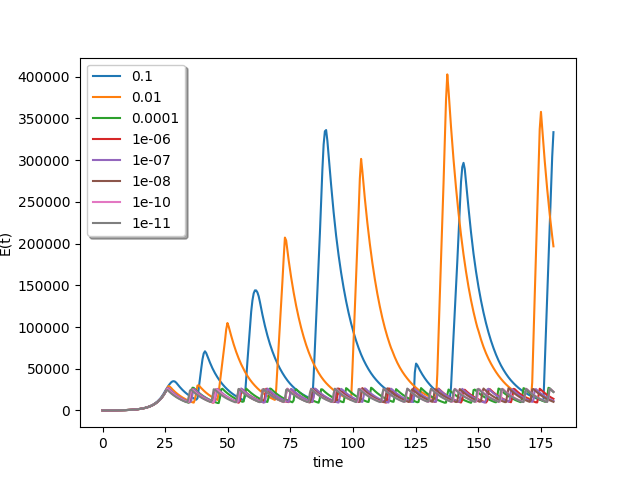
\includegraphics[width=0.7\linewidth]{./figures/exp_state_tol_lsoda_no_event_10}
\caption{State-dependent discontinuity model tolerance study on the Python version of LSODA without event detection with a steepness of change of 10.}
\label{fig:exp_state_tol_lsoda_no_event_10}
\end{figure}

\begin{figure}[H]
\centering
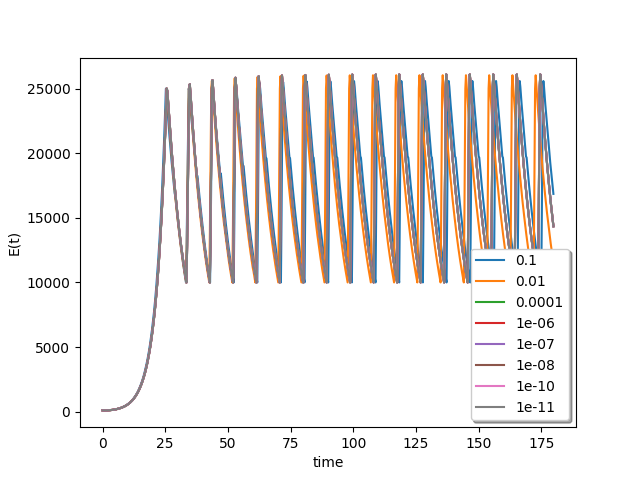
\includegraphics[width=0.7\linewidth]{./figures/exp_state_tol_lsoda_event_10}
\caption{State-dependent discontinuity model tolerance study on the Python version of LSODA with event detection with a steepness of change of 10.}
\label{fig:exp_state_tol_lsoda_event_10}
\end{figure}

\begin{table}[H]
\caption {Python LSODA state-dependent discontinuity model with exponential change with a steepness of change of 10 tolerance study - number of function evaluations} \label{tab:exp_state_tol_lsoda_10} 
\begin{center}
\begin{tabular}{ c c c }
tolerance & no event detection & with event detection \\ 
0.1 & 365 & 763 \\
0.01 & 504 & 878 \\
0.0001 & 2338 & 1746 \\
1e-06 & 4004 & 3106 \\
1e-07 & 5224 & 4004 \\
1e-08 & 6158 & 4984 \\
1e-10 & 8565 & 7367 \\
1e-11 & 10068 & 7885 \\
\end{tabular}
\end{center}
\end{table}



\subsubsection{RK45 state-dependent discontinuity problem tolerance study}
\paragraph{steepness of change of 0.1}

\begin{figure}[H]
\centering
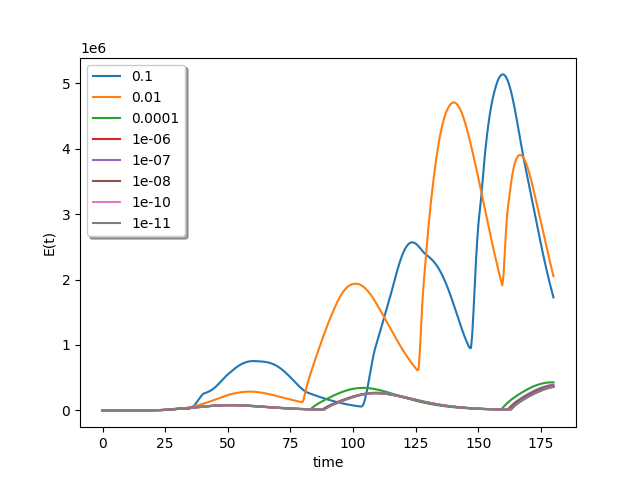
\includegraphics[width=0.7\linewidth]{./figures/exp_state_tol_rk45_no_event_0_1}
\caption{State-dependent discontinuity model tolerance study on the Python version of RK45 without event detection with a steepness of change of 0.1.}
\label{fig:exp_state_tol_rk45_no_event_0_1}
\end{figure}

\begin{figure}[H]
\centering
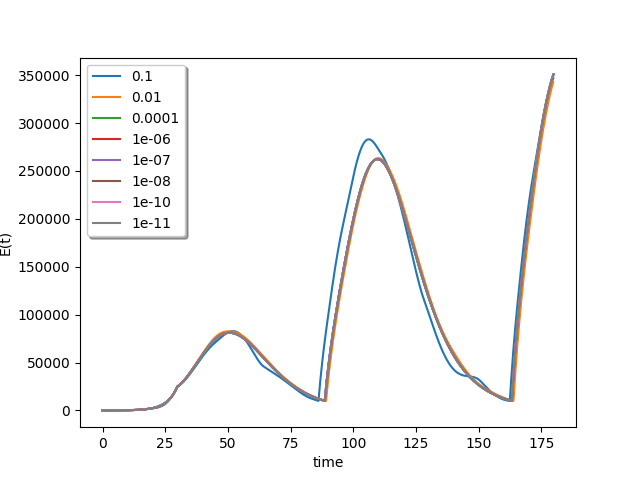
\includegraphics[width=0.7\linewidth]{./figures/exp_state_tol_rk45_event_0_1}
\caption{State-dependent discontinuity model tolerance study on the Python version of RK45 with event detection with a steepness of change of 0.1.}
\label{fig:exp_state_tol_rk45_event_0_1}
\end{figure}

\begin{table}[H]
\caption {Python RK45 state-dependent discontinuity model with exponential change with a steepness of change of 0.1 tolerance study - number of function evaluations} \label{tab:exp_state_tol_rk45_0_1} 
\begin{center}
\begin{tabular}{ c c c }
tolerance & no event detection & with event detection \\ 
0.1 & 164 & 180 \\
0.01 & 224 & 222 \\
0.0001 & 458 & 360 \\
1e-06 & 1094 & 726 \\
1e-07 & 1490 & 1062 \\
1e-08 & 2066 & 1608 \\
1e-10 & 4430 & 3834 \\
1e-11 & 6644 & 6006 \\
\end{tabular}
\end{center}
\end{table}

\paragraph{steepness of change of 1}
\begin{figure}[H]
\centering
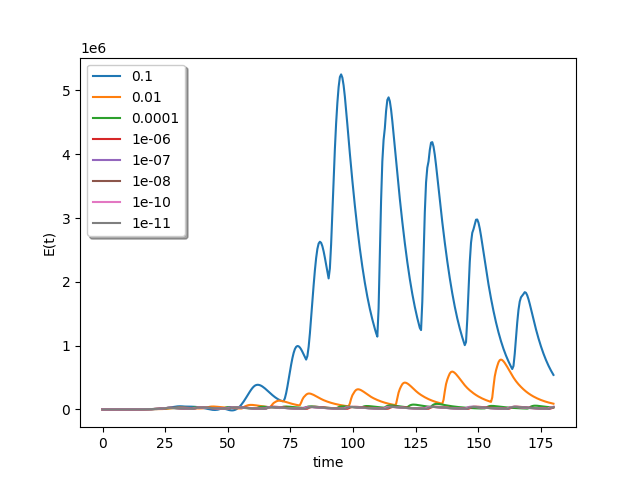
\includegraphics[width=0.7\linewidth]{./figures/exp_state_tol_rk45_no_event_1}
\caption{State-dependent discontinuity model tolerance study on the Python version of RK45 without event detection with a steepness of change of 1.}
\label{fig:exp_state_tol_rk45_no_event_1}
\end{figure}

\begin{figure}[H]
\centering
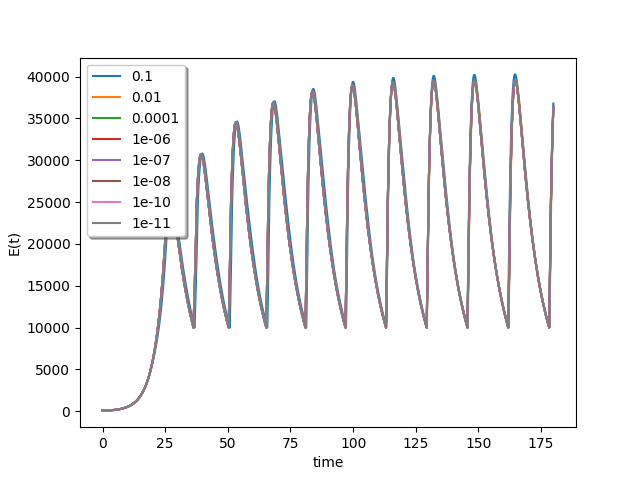
\includegraphics[width=0.7\linewidth]{./figures/exp_state_tol_rk45_event_1}
\caption{State-dependent discontinuity model tolerance study on the Python version of RK45 with event detection with a steepness of change of 1.}
\label{fig:exp_state_tol_rk45_event_1}
\end{figure}

\begin{table}[H]
\caption {Python RK45 state-dependent discontinuity model with exponential change with a steepness of change of 1 tolerance study - number of function evaluations} \label{tab:exp_state_tol_lsoda_1} 
\begin{center}
\begin{tabular}{ c c c }
tolerance & no event detection & with event detection \\ 
0.1 & 320 & 434 \\
0.01 & 416 & 452 \\
0.0001 & 1100 & 776 \\
1e-06 & 2738 & 1166 \\
1e-07 & 3506 & 1658 \\
1e-08 & 4490 & 2378 \\
1e-10 & 7898 & 5306 \\
1e-11 & 11042 & 8126 \\
\end{tabular}
\end{center}
\end{table}



\paragraph{steepness of change of 10}
\begin{figure}[H]
\centering
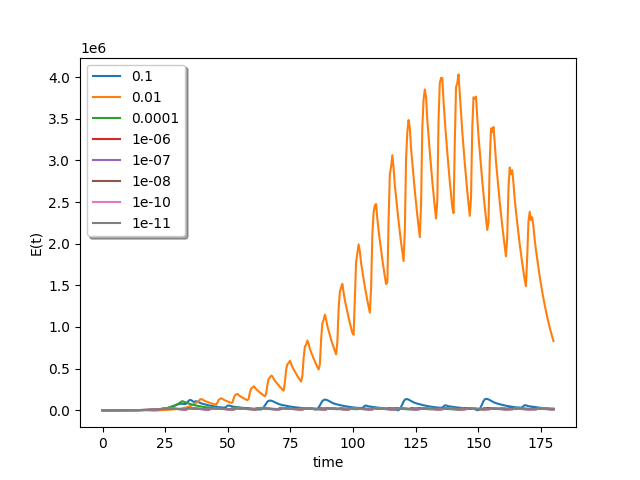
\includegraphics[width=0.7\linewidth]{./figures/exp_state_tol_rk45_no_event_10}
\caption{State-dependent discontinuity model tolerance study on the Python version of RK45 without event detection with a steepness of change of 10.}
\label{fig:exp_state_tol_rk45_no_event_10}
\end{figure}

\begin{figure}[H]
\centering
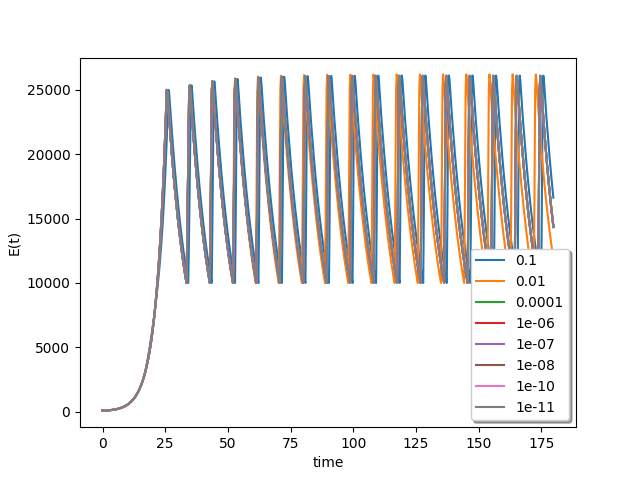
\includegraphics[width=0.7\linewidth]{./figures/exp_state_tol_rk45_event_10}
\caption{State-dependent discontinuity model tolerance study on the Python version of RK45 with event detection with a steepness of change of 10.}
\label{fig:exp_state_tol_rk45_event_10}
\end{figure}

\begin{table}[H]
\caption {Python RK45 state-dependent discontinuity model with exponential change with a steepness of change of 10 tolerance study - number of function evaluations} \label{tab:exp_state_tol_rk45_10} 
\begin{center}
\begin{tabular}{ c c c }
tolerance & no event detection & with event detection \\ 
0.1 & 410 & 674 \\
0.01 & 776 & 710 \\
0.0001 & 1346 & 1040 \\
1e-06 & 3686 & 2024 \\
1e-07 & 5402 & 2756 \\
1e-08 & 8036 & 4046 \\
1e-10 & 13574 & 8978 \\
1e-11 & 18476 & 13400 \\
\end{tabular}
\end{center}
\end{table}


